% Created by tikzDevice version 0.6.2-92-0ad2792 on 2013-04-07 17:58:07
% !TEX encoding = UTF-8 Unicode
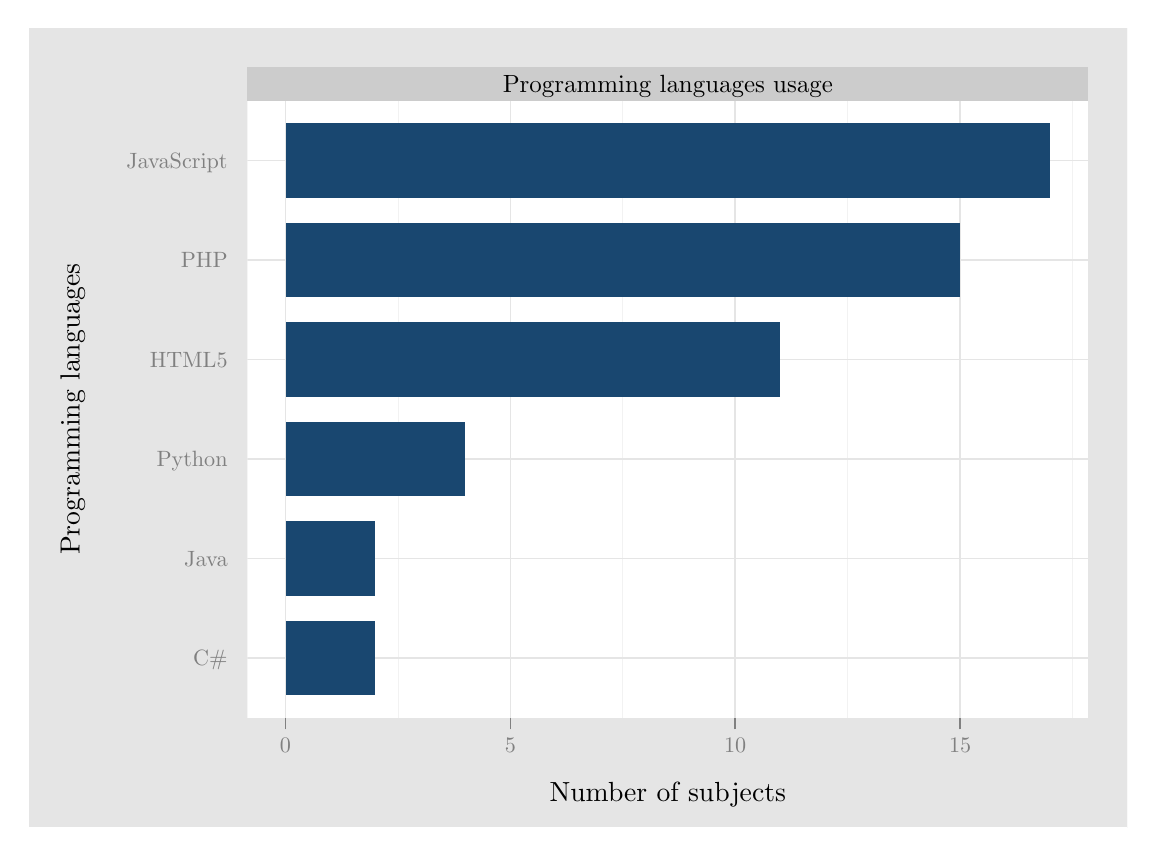
\begin{tikzpicture}[x=1pt,y=1pt]
\definecolor[named]{fillColor}{rgb}{1.00,1.00,1.00}
\path[use as bounding box,fill=fillColor,fill opacity=0.00] (0,0) rectangle (397.48,289.08);
\begin{scope}
\path[clip] (  0.00,  0.00) rectangle (397.48,289.08);
\definecolor[named]{drawColor}{rgb}{1.00,1.00,1.00}
\definecolor[named]{fillColor}{rgb}{0.90,0.90,0.90}

\path[draw=drawColor,line width= 0.6pt,line join=round,line cap=round,fill=fillColor] (  0.00, -0.00) rectangle (397.48,289.08);
\end{scope}
\begin{scope}
\path[clip] ( 79.35, 39.76) rectangle (383.26,262.63);
\definecolor[named]{fillColor}{rgb}{1.00,1.00,1.00}

\path[fill=fillColor] ( 79.35, 39.76) rectangle (383.26,262.63);
\definecolor[named]{drawColor}{rgb}{0.95,0.95,0.95}

\path[draw=drawColor,line width= 0.3pt,line join=round] (133.80, 39.76) --
	(133.80,262.63);

\path[draw=drawColor,line width= 0.3pt,line join=round] (215.05, 39.76) --
	(215.05,262.63);

\path[draw=drawColor,line width= 0.3pt,line join=round] (296.31, 39.76) --
	(296.31,262.63);

\path[draw=drawColor,line width= 0.3pt,line join=round] (377.57, 39.76) --
	(377.57,262.63);
\definecolor[named]{drawColor}{rgb}{0.90,0.90,0.90}

\path[draw=drawColor,line width= 0.6pt,line join=round] ( 79.35, 61.33) --
	(383.26, 61.33);

\path[draw=drawColor,line width= 0.6pt,line join=round] ( 79.35, 97.27) --
	(383.26, 97.27);

\path[draw=drawColor,line width= 0.6pt,line join=round] ( 79.35,133.22) --
	(383.26,133.22);

\path[draw=drawColor,line width= 0.6pt,line join=round] ( 79.35,169.17) --
	(383.26,169.17);

\path[draw=drawColor,line width= 0.6pt,line join=round] ( 79.35,205.12) --
	(383.26,205.12);

\path[draw=drawColor,line width= 0.6pt,line join=round] ( 79.35,241.06) --
	(383.26,241.06);

\path[draw=drawColor,line width= 0.6pt,line join=round] ( 93.17, 39.76) --
	( 93.17,262.63);

\path[draw=drawColor,line width= 0.6pt,line join=round] (174.43, 39.76) --
	(174.43,262.63);

\path[draw=drawColor,line width= 0.6pt,line join=round] (255.68, 39.76) --
	(255.68,262.63);

\path[draw=drawColor,line width= 0.6pt,line join=round] (336.94, 39.76) --
	(336.94,262.63);
\definecolor[named]{fillColor}{rgb}{0.10,0.28,0.44}

\path[fill=fillColor] ( 93.17, 47.85) rectangle (125.67, 74.81);

\path[fill=fillColor] ( 93.17, 83.79) rectangle (125.67,110.76);

\path[fill=fillColor] ( 93.17,119.74) rectangle (158.17,146.70);

\path[fill=fillColor] ( 93.17,155.69) rectangle (271.94,182.65);

\path[fill=fillColor] ( 93.17,191.64) rectangle (336.94,218.60);

\path[fill=fillColor] ( 93.17,227.58) rectangle (369.44,254.54);
\end{scope}
\begin{scope}
\path[clip] (  0.00,  0.00) rectangle (397.48,289.08);
\definecolor[named]{fillColor}{rgb}{0.80,0.80,0.80}

\path[fill=fillColor] ( 79.35,262.63) rectangle (383.26,274.85);
\definecolor[named]{drawColor}{rgb}{0.00,0.00,0.00}

\node[text=drawColor,anchor=base,inner sep=0pt, outer sep=0pt, scale=  0.90] at (231.31,265.64) {Programming languages usage};
\end{scope}
\begin{scope}
\path[clip] (  0.00,  0.00) rectangle (397.48,289.08);
\definecolor[named]{drawColor}{rgb}{0.50,0.50,0.50}

\node[text=drawColor,anchor=base east,inner sep=0pt, outer sep=0pt, scale=  0.80] at ( 72.24, 58.57) {C\#};

\node[text=drawColor,anchor=base east,inner sep=0pt, outer sep=0pt, scale=  0.80] at ( 72.24, 94.52) {Java};

\node[text=drawColor,anchor=base east,inner sep=0pt, outer sep=0pt, scale=  0.80] at ( 72.24,130.47) {Python};

\node[text=drawColor,anchor=base east,inner sep=0pt, outer sep=0pt, scale=  0.80] at ( 72.24,166.41) {HTML5};

\node[text=drawColor,anchor=base east,inner sep=0pt, outer sep=0pt, scale=  0.80] at ( 72.24,202.36) {PHP};

\node[text=drawColor,anchor=base east,inner sep=0pt, outer sep=0pt, scale=  0.80] at ( 72.24,238.31) {JavaScript};
\end{scope}
\begin{scope}
\path[clip] (  0.00,  0.00) rectangle (397.48,289.08);
\definecolor[named]{drawColor}{rgb}{0.50,0.50,0.50}

\path[draw=drawColor,line width= 0.6pt,line join=round] ( 93.17, 35.49) --
	( 93.17, 39.76);

\path[draw=drawColor,line width= 0.6pt,line join=round] (174.43, 35.49) --
	(174.43, 39.76);

\path[draw=drawColor,line width= 0.6pt,line join=round] (255.68, 35.49) --
	(255.68, 39.76);

\path[draw=drawColor,line width= 0.6pt,line join=round] (336.94, 35.49) --
	(336.94, 39.76);
\end{scope}
\begin{scope}
\path[clip] (  0.00,  0.00) rectangle (397.48,289.08);
\definecolor[named]{drawColor}{rgb}{0.50,0.50,0.50}

\node[text=drawColor,anchor=base,inner sep=0pt, outer sep=0pt, scale=  0.80] at ( 93.17, 27.14) {0};

\node[text=drawColor,anchor=base,inner sep=0pt, outer sep=0pt, scale=  0.80] at (174.43, 27.14) {5};

\node[text=drawColor,anchor=base,inner sep=0pt, outer sep=0pt, scale=  0.80] at (255.68, 27.14) {10};

\node[text=drawColor,anchor=base,inner sep=0pt, outer sep=0pt, scale=  0.80] at (336.94, 27.14) {15};
\end{scope}
\begin{scope}
\path[clip] (  0.00,  0.00) rectangle (397.48,289.08);
\definecolor[named]{drawColor}{rgb}{0.00,0.00,0.00}

\node[text=drawColor,anchor=base,inner sep=0pt, outer sep=0pt, scale=  1.00] at (231.31,  9.41) {Number of subjects};
\end{scope}
\begin{scope}
\path[clip] (  0.00,  0.00) rectangle (397.48,289.08);
\definecolor[named]{drawColor}{rgb}{0.00,0.00,0.00}

\node[text=drawColor,rotate= 90.00,anchor=base,inner sep=0pt, outer sep=0pt, scale=  1.00] at ( 18.80,151.20) {Programming languages};
\end{scope}
\end{tikzpicture}
